\section{Opis implementacije praktičnog rada}

\subsection{Instalacija i konfiguracija okruženja}

\subsubsection{Početni komplet Laravel Jetstream}
Kako bi developerima uštedio vrijeme u samome početku razvijanja nove aplikacije, Laravel nudi autentikacijske i aplikacijske početne komplete (engl.~\textit{starter kits}) kao što su Laravel Breeze i Laravel Jetstream koji automatski pružaju rute, kontrolere i poglede (engl. \textit{views}) potrebne za registraciju i autentikaciju~\cite{starterKits}.

Laravel Jetstream dizajniran je koristeći \textbf{Tailwind CSS}, \textit{utility-first} CSS razvojni okvir. Datoteke \texttt{postcss.config.js} i \texttt{tailwind.config.js} koriste pri \textit{buildanju} kompajliranog CSS-a aplikacije.

Značajke koje Laravel Jetstream početni komplet pruža su autentikacija, registracija, upravljanje korisničkim profilima, ponovno postavljanje lozinke, verifikacija e-adrese, dvostruka provjera autentičnosti (engl. \textit{two-factor authentication}), upravljanje aktivnim sesijama u web preglednicima, API podrška te opcionalne opcije za upravljanje timovima~\cite{jetstreamIntro}.

Instalira se koristeći Composer, a naredbe za instalaciju prikazane su ispisu~\ref{jetstreamInstallation}.

\begin{lstlisting}[caption={Naredbe za instalaciju Jetstream paketa u novi Laravel projekt}, label=jetstreamInstallation]
composer create-project laravel/laravel teamstructor-app

cd teamstructor-app

composer require laravel/jetstream
\end{lstlisting}

Jetstream pruža izbor između korištenja \textbf{Livewire} ili Inertia.js \textit{frontend scaffoldinga}. O tom izboru ovisi i odabrani jezik za predloške (engl. \textit{templating language}) jer uz Livewire to je \textbf{Blade}, a uz Inertia.js to je Vue.js~\cite{jetstreamIntro}. \\ Za instaliranje Jetstreama s Livewire \textit{frontend scaffoldingom} i to s uključenom podrškom za timove koristi se naredba \texttt{php artisan jetstream:install livewire -{}-teams}~\cite{jetstreamInstallation}.

\texttt{php artisan vendor:publish -{}-tag=jetstream-views} je naredba čijim se izvršavanjem u \texttt{app} direktoriju kreira direktorij \texttt{resources/view/components} koji sadrži razne generičke Blade komponente čija je svrha da ih se jednostavno može koristiti te pružanje konzistentnog korisničkog sučelja bez potrebe da developer kreira vlastite komponente~\cite{jetstreamLivewire}.

Nakon instalacije Jetstreama potrebno je instalirati i pokrenuti \textit{build} NPM ovisnosti pomoću naredbi \texttt{npm install} i \texttt{npm run build} te migrirati bazu naredbom \texttt{php artisan migrate}~\cite{jetstreamInstallation}.

\subsubsection{\texttt{.env} datoteka}
\texttt{.env} datoteka nalazi se u aplikacijskom root direktoriju i služi kao konfiguracijska datoteka za Laravel web aplikaciju. Pri instalaciji Laravela kreirana je tako da se u nju kopira ogledna konfiguracijska datoteka \texttt{.env.example}~\cite{configuration}. 

Dobra je praksa i zbog sigurnosti i zbog toga što je konfiguracija promjenjiva ovisno o pojedinačnim okruženjima da neenkriptirana \texttt{.env} datoteka nije dio kontrole izvornog k\^oda aplikacije, dok je to u redu za \texttt{.env.example} datoteku te ista može poslužiti kao ogledni primjer s \textit{placeholder} vrijednostima za varijable koje je potrebno definirati~\cite{configuration}.

Primjer definicije varijable može se vidjeti u ispisu~\ref{envDefinition}.

\begin{lstlisting}[caption={Definicija varijable u \texttt{.env datoteci}}, label=envDefinition]
APP_NAME=Teamstructor
\end{lstlisting}

U Laravel aplikaciji pristup vrijednosti pojedine varijable iz \texttt{.env} datoteke moguć je pomoću \texttt{\$\_ENV} PHP superglobalne varijable ili koristeći funkciju \texttt{env}, kao u ispisu~\ref{envRetrieve}.

\begin{lstlisting}[caption={Pristup vrijednosti \textit{environment} varijable u Laravelu}, label=envRetrieve]
'name' => env('APP_NAME', 'Laravel'),
\end{lstlisting}

\subsection{Struktura Laravel aplikacije}

\subsubsection{Struktura početnog direktorija s izvornim k\^odom aplikacije}
Osnovna struktura \textit{root} direktorija Laravel aplikacije jest sljedeća~\cite{structure}:  \\
\dirtree{%
.1 teamstructor-app.
.2 app.
.2 bootstrap.
.2 config.
.2 database.
.2 node\_modules.
.2 public.
.2 resources.
.2 routes.
.2 storage.
.2 tests.
.2 vendor.
}

\begin{itemize}
\item \texttt{app} - Sadrži "jezgru" aplikacije te će biti posebno predstavljen u poglavlju~\ref{subsubsection:app}.
\item \texttt{bootstrap} - Sadrži datoteku \texttt{app.php} koja pokreće razvojni okvir te direktorij \texttt{cache} koji sadrži datoteke predmemorije za optimizaciju performansi.
\item \texttt{config} - Sadrži konfiguracijske datoteke.
\item \texttt{database} - Sadrži migracije, tvornice modela (engl. \textit{model factories}) i \textit{seed}-ove.
\item \texttt{node\_modules} - Nije u osnovnoj strukturi, međutim nastaje instalacijom NPM ovisnosti te sadrži instalirane module tj. biblioteke potrebne za \textit{frontend} dio aplikacije kao poddirektorije.
\item \texttt{public} - Sadrži datoteku \texttt{index.php} koja je polazna točka svih zahtjeva prema aplikaciji te konfigurira automatsko učitavanje (engl. \textit{autoloading}).  Također se tu nalaze i javna "imovina" aplikacije (engl. \textit{assets}): slike te JavaScript i CSS datoteke.
\item \texttt{resources} - Sadrži poglede (engl. \textit{views}) i nekompajlirane JavaScript i CSS datoteke koje su \textit{assets} aplikacije.
\item \texttt{routes} - Sadrži definicije svih ruta u aplikaciji. Zadano su uključene datoteke: \texttt{web.php}, \texttt{api.php}, \texttt{console.php} i \texttt{channels.php}.
\item \texttt{storage} - Služi kao lokalno spremište podataka aplikacije te je podijeljen na direktorije \texttt{app}, \texttt{framework} i \texttt{logs}. Sadrži \texttt{.log} datoteke zapisnika, kompajlirane Blade predloške, sesije, predmemorije datoteka itd.
\item \texttt{tests} - Sadrži skripte za automatizirane testove aplikacije te dolazi s po jednim oglednim primjerom \textit{unit} i \textit{feature} testova.
\item \texttt{vendor} - Sadrži preuzete Composer ovisnosti aplikacije.
\end{itemize}

\subsubsection{Struktura \texttt{app} direktorija}
\label{subsubsection:app}
Na slici~\ref{fig:appDir} prikazan je sadržaj \texttt{app} direktorija.
\begin{figure}[H]
	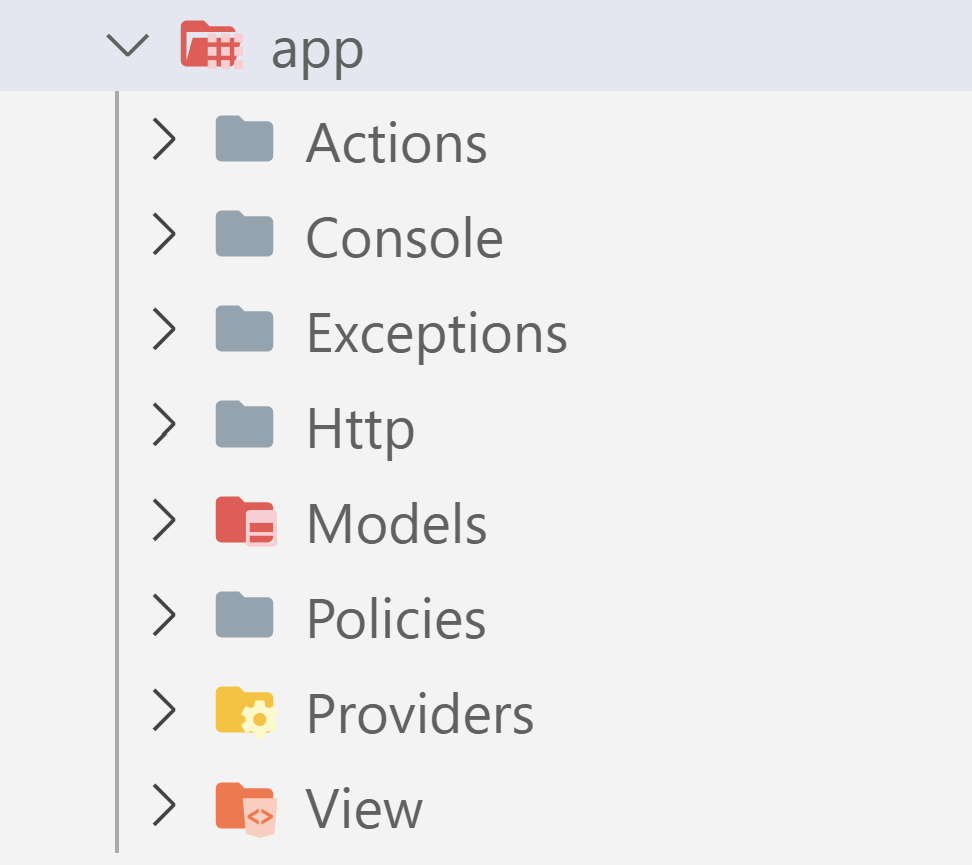
\includegraphics[width=0.4\linewidth,clip=]{assets/app-directory.png}
	\centering
	\caption{Sadržaj \texttt{app} direktorija}
	\label{fig:appDir}
\end{figure}

Možemo vidjeti da se \texttt{app} direktorij sastoji od sljedećih poddirektorija~\cite{structure}: 
\begin{itemize}
\item \texttt{Actions} - Direktorij koji se kreira pri Jetstream instalaciji, a sadrži \texttt{Action} klase koje obično izvode samo jednu akciju i odgovaraju jednoj Jetstream ili Fortify značajki kao npr. kreiranje korisnika ili tima,  postavljanje nove lozinke, brisanje korisnika ili tima, dodavanje člana u tim itd.~\cite{jetstreamActions}
\item \texttt{Console} - Sadrži datoteku \texttt{Kernel.php} u kojoj se registriraju \textit{custom} Artisan naredbe.
\item \texttt{Exceptions} - Sadrži datoteku \texttt{Handler.php} koja upravlja svim iznimkama u aplikaciji te je moguće registrirati nove \textit{custom} iznimke.
\item \texttt{Http} - Gotovo sva logika aplikacije smještena je u ovaj direktorij. Sadrži kontrolere, klase Livewire komponenti te \textit{middleware}.
\item \texttt{Models} - Sadrži klase svih Eloquent modela ove web aplikacije.
\item \texttt{Policies} - Nastaje izvođenjem \texttt{make:policy} Artisan naredbe te sadrži klase u kojima su definirana pravila autorizacije unutar aplikacije.
\item \texttt{Providers} - Sadrži sve davatelje usluga (engl. \textit{service providers}) aplikacije.
\item \texttt{View} - Direktorij se kreira pri Jetstream instalaciji, a sadrži klase Livewire \textit{layout} komponenti - "application" \textit{layout} te "guest" \textit{layout}~\cite{jetstreamLayouts}.
\end{itemize}

Još nekolicina direktorija može biti generirana unutar \texttt{app} direktorija izvršavanjem Artisan \texttt{make} naredbi za generiranje klasa~\cite{structure}. 

\subsection{Struktura relacijske baze podataka}
Na slici~\ref{fig:erDiagram} prikazan je ER (engl. \textit{Entity Relationship}) dijagram relacijske baze podataka u phpMyAdmin sučelju na kojemu možemo vidjeti tablice u koje su podatci spremani te njihove međusobne relacije.
\begin{figure}[H]
	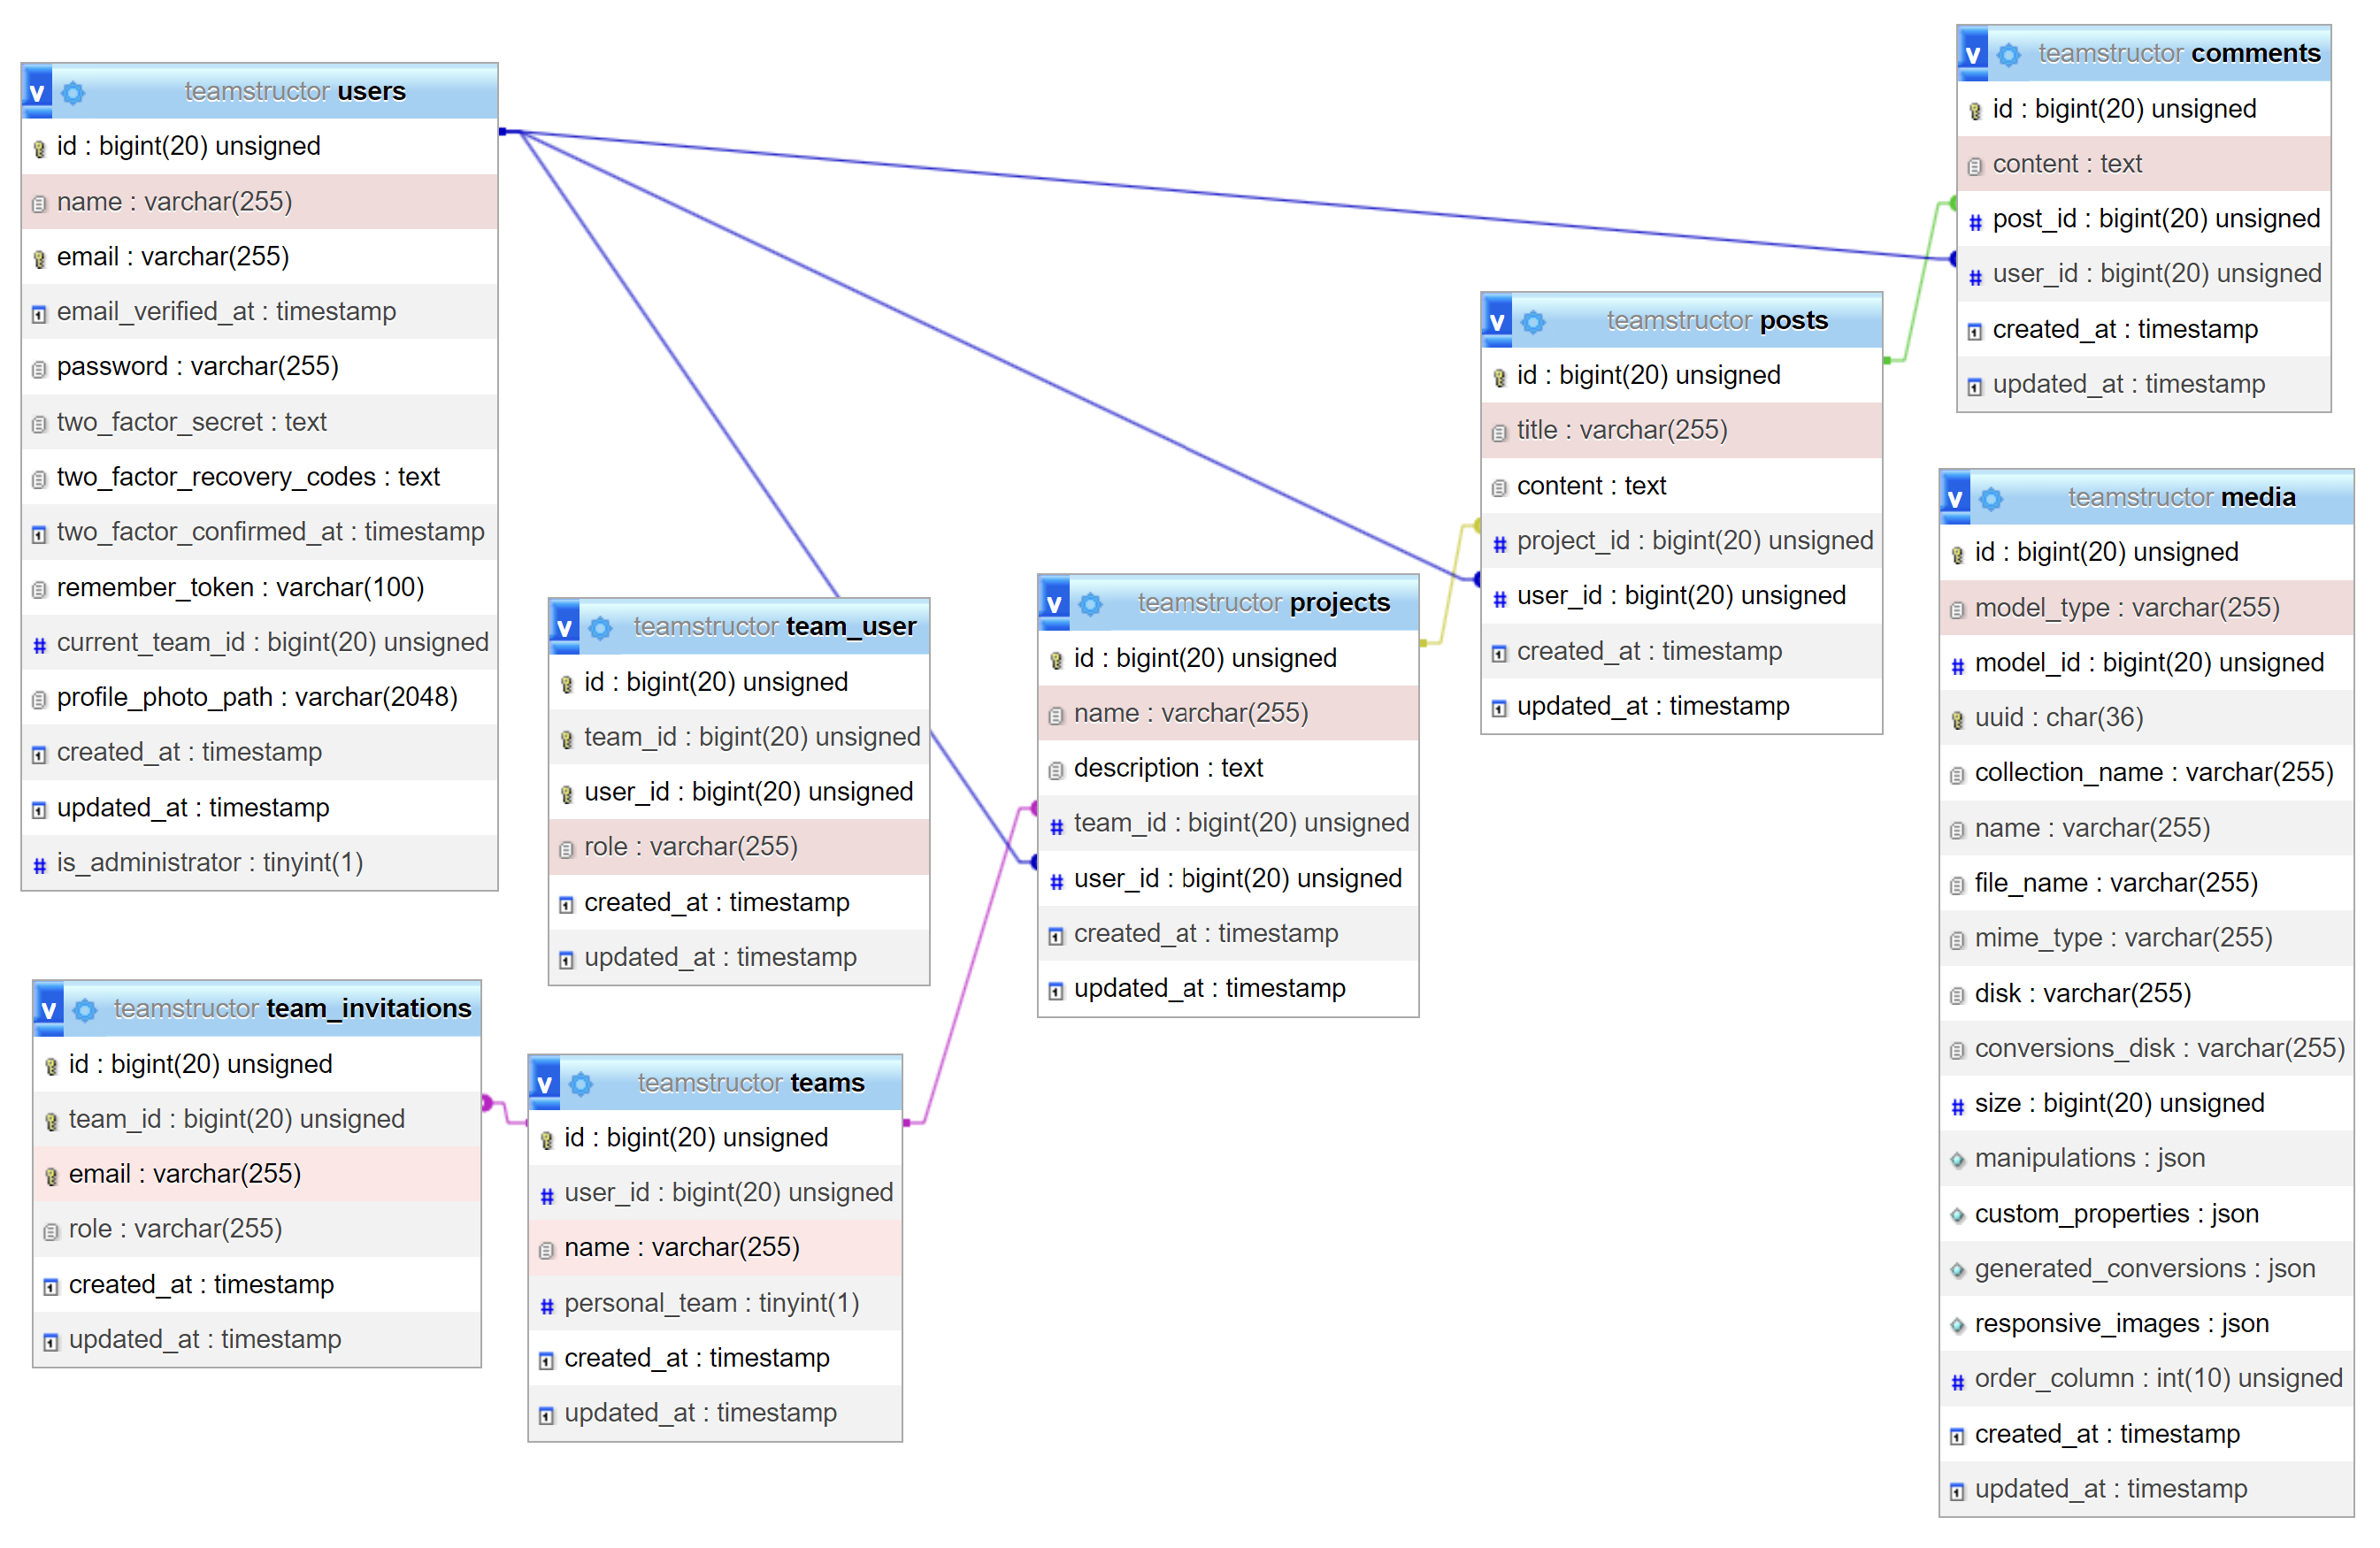
\includegraphics[width=1\linewidth,clip=]{assets/db-er-diagram.png}
	\centering
	\caption{Dijagram relacijske baze podataka}
	\label{fig:erDiagram}
\end{figure}

Radi preglednosti su na dijagramu sa slike~\ref{fig:erDiagram} prikazane samo tablice koje se odnose na modele, a izostavljene su tablice: 
\begin{itemize}
\item \texttt{failed\_jobs} - Automatski prisutna u Laravel aplikacijama, služi za pohranu poslova iz reda čekanja koji se nisu uspjeli izvršiti.
\item \texttt{migrations} - Automatski prisutna u Laravel aplikacijama, služi za pohranu migracija.
\item \texttt{password\_reset\_tokens} - Automatski prisutna u Laravel aplikacijama, služi za pohranu tokena za ponovno postavljanje lozinki u aplikaciji.
\item \texttt{personal\_access\_tokens} - Kreira ju Laravel Sanctum pri instalaciji Laravel Jetstreama, a služi za pohranu API tokena u aplikaciji.
\item \texttt{sessions} - Kada se koristi \texttt{database} \textit{driver} za sesije, onda se u ovu tablicu iste pohranjuju.
\item \texttt{telescope\_entries}, \texttt{telescope\_entries\_tags}, \texttt{telescope\_monitoring} - Nastaju pri instalaciji Laravel Telescopea, a služe za pohranu podataka za Telescope.
\end{itemize}

U poglavlju~\ref{subsubsection:dbInteraction} će biti više rečeno o načinima na koje se ostvaruje interakcija s bazom podataka te o samim modelima i relacijama.

\subsection{Interakcija s bazom podataka}
\label{subsubsection:dbInteraction}

\subsubsection{Migracije}
Migracije služe kao kontrola verzije baze podataka. U Laravelu migracije koriste fasadu (engl. \textit{facade}) \texttt{Schema} koja pruža \textit{database agnostic} podršku za sve sustave baza podataka koje Laravel podržava.

Migracija se može kreirati pozivom \texttt{make:migration} Artisan naredbe te će se ista smjestiti u \texttt{database/migrations} direktorij. Nazivu svake migracije dodaje se pripadajući \textit{timestamp} prema kojem Laravel prati redoslijed migracija.

Sama migracijska klasa sadrži dvije metode: \texttt{up} koja kreira ili modificira tablice, stupce ili indekse u bazi podataka te \texttt{down} koja bi trebala poništiti promjene učinjene u \texttt{up} metodi inverznim operacijama.

U ispisu~\ref{projectsTableMigration} možemo vidjeti k\^od migracije za kreiranje tablice \texttt{projects} u kojoj u \texttt{up} metodi kreiramo tablicu navodeći njezin naziv i stupce koje sadrži, a u \texttt{down} metodi poništavamo operacije izvedene u \texttt{up} metodi na način da se odbacuje novokreirana tablica tj. izvodi \textit{drop} tablice.

\begin{lstlisting}[caption={Migracija za kreiranje tablice \texttt{projects}}, label=projectsTableMigration]
<?php

use Illuminate\Database\Migrations\Migration;
use Illuminate\Database\Schema\Blueprint;
use Illuminate\Support\Facades\Schema;

return new class extends Migration
{
    /**
     * Run the migrations.
     */
    public function up(): void
    {
        Schema::create('projects', function (Blueprint $table) {
            $table->id();
            $table->string('name');
            $table->text('description');
            $table->foreignId('team_id')->constrained();
            $table->foreignId('user_id')->constrained();
            $table->timestamps();
        });
    }

    /**
     * Reverse the migrations.
     */
    public function down(): void
    {
        Schema::dropIfExists('projects');
    }
};

\end{lstlisting}

U ispisu~\ref{administratorColumnMigration} prikazana je migracija koja modificira tablicu \texttt{users} tako da joj dodaje stupac \texttt{is\_administrator}. U \texttt{up} metodi definira se stupac koji će se dodati, a u \texttt{down} metodi te promjene će biti poništene odbacivanjem novododanog stupca metodom \texttt{dropColumn}.

\begin{lstlisting}[caption={Migracija za dodavanje stupca \texttt{is\_administrator} u tablicu \texttt{users}}, label=administratorColumnMigration]
<?php

use Illuminate\Database\Migrations\Migration;
use Illuminate\Database\Schema\Blueprint;
use Illuminate\Support\Facades\Schema;

return new class extends Migration
{
    /**
     * Run the migrations.
     */
    public function up(): void
    {
        Schema::table('users', function (Blueprint $table) {
            $table->boolean('is_administrator')->default(false);
        });
    }

    /**
     * Reverse the migrations.
     */
    public function down(): void
    {
        Schema::table('users', function (Blueprint $table) {
            $table->dropColumn('is_administrator');
        });
    }
};

\end{lstlisting}

Za izvršiti sve migracije koje se još nisu primjenile na bazu podataka pokreće se Artisan naredba \texttt{migrate}, a za povratak na prethodnu migraciju tj. poništavanje promjena posljednjih \textit{n} migracija Artisan naredba \texttt{migrate:rollback}.

\subsubsection{Populacija podatcima (engl. \textit{seeding})}

\subsubsection{Eloquent ORM}

\paragraph{Modeli i tvornice modela (engl. \textit{model factories})}

\paragraph{Relacije}

\paragraph{Query Builder i kolekcije}

\subsection{Usmjerivanje zahtjeva (engl. \textit{routing})}

\subsection{Middleware}

\subsection{Autentikacija}

\subsection{Autorizacija}

\subsubsection{Politike (engl. \textit{policies})}

\subsubsection{Vrata (engl. \textit{gates})}

\subsection{Livewire komponente}

\subsubsection{Akcije}

\subsubsection{Događaji}

\subsection{Pohrana datoteka}

\subsubsection{MinIO - AWS S3 kompatibilan servis za pohranu}

\subsection{Spatie Laravel Media Library paket}

\subsection{Lokalizacija}

\subsection{Testiranje i kvaliteta k\^oda}

\subsubsection{Korišteni alati}

\paragraph{Laravel Debug Bar}

\paragraph{Laravel Telescope}

\paragraph{Laravel Pint}

\subsubsection{Pretpregled elektroničke pošte - MailHog}

\subsubsection{Pisanje i pokretanje testova}

\subsection{Otvoreni k\^od i doprinos zajednice na projektima Laravel ekosustava}
